\begin{figure}[!htb]
  \centering
  \caption{Transition Maps (No Saving)}
  \begin{minipage}[t]{0.4\textwidth}
    \centering
    \small{(a) $\Delta$ Mean Welfare (CE)}
    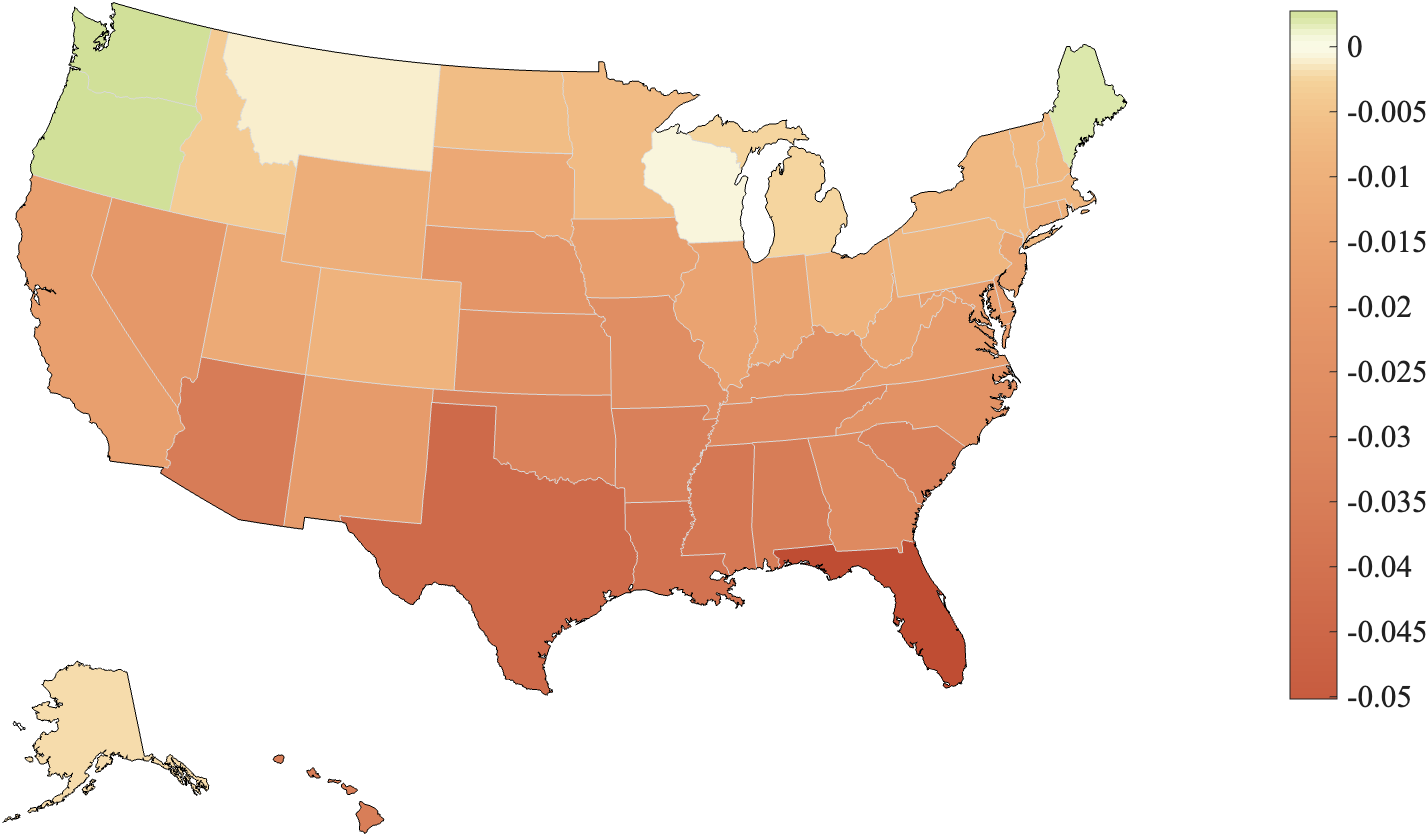
\includegraphics[width=\textwidth]{../Output/big_nu/graph_no_saving_struct/transition_maps/transition_maps_delta_mean_welfare_ce.png}
  \end{minipage}\hfill
  \begin{minipage}[t]{0.4\textwidth}
    \centering
    \small{(b) $\Delta$ Local Population (\%)}
    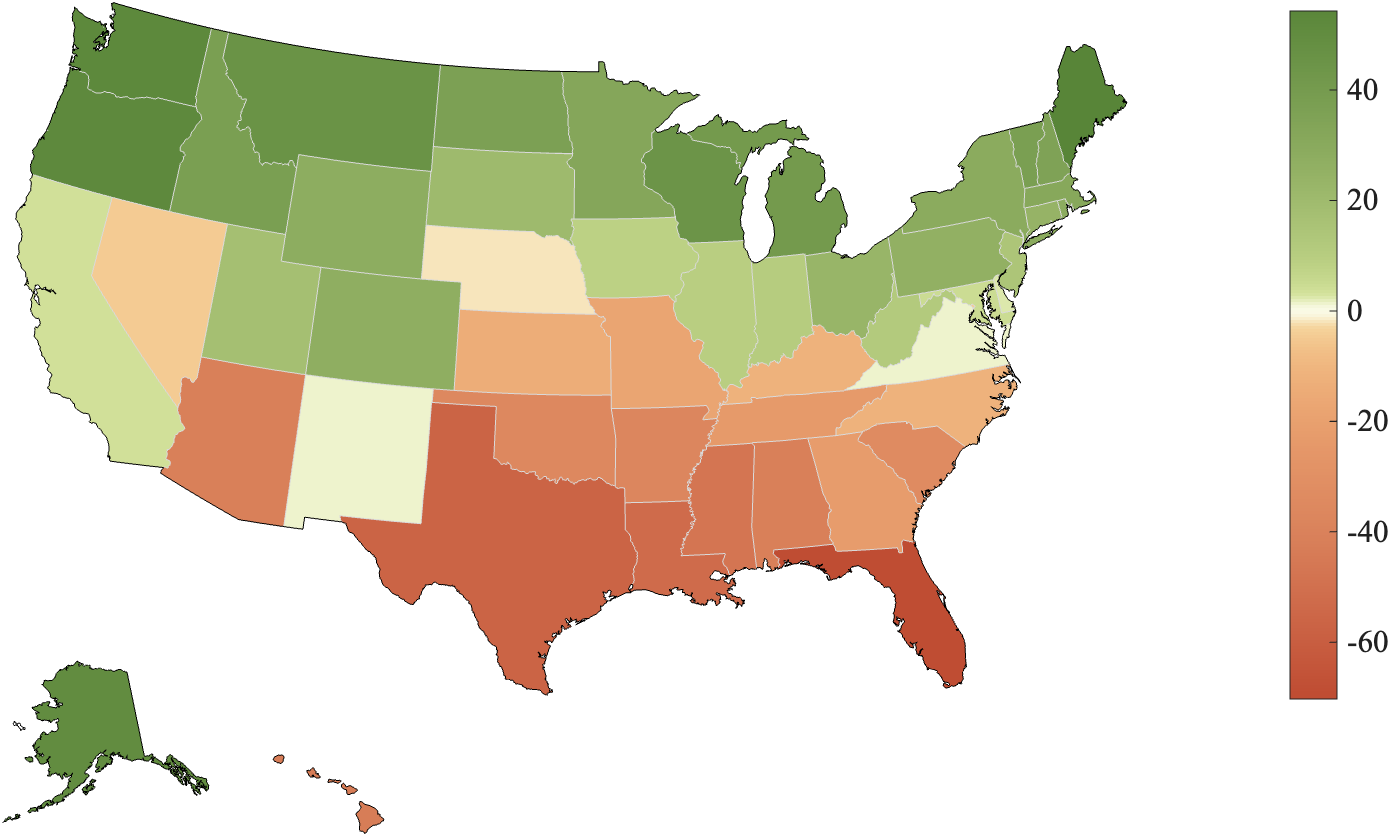
\includegraphics[width=\textwidth]{../Output/big_nu/graph_no_saving_struct/transition_maps/transition_maps_local_pop_changes_pct.png}
  \end{minipage}\hfill
  \begin{minipage}{\textwidth}
  \vspace{0.5em}
  \footnotesize{\textbf{Note:} Spatial maps comparing the terminal steady state under 2100 climate parameters ($SS_\text{term}$) to the initial 2010 baseline steady state ($SS_\text{init}$) under Hand-to-Mouth workers. Panel (a): change in mean Certainty Equivalent welfare $\Delta \text{CE}_\ell = \overline{\Xi}_{\ell, \text{term}}^{\text{NS}} - \overline{\Xi}_{\ell, \text{init}}^{\text{NS}}$, which collapses strictly to non-asset value index $\Xi^{\text{NS}}$. Panel (b): relative population percentage change $\Delta L_\ell\% = 100 \times (L_{\ell, \text{term}} - L_{\ell, \text{init}})/L_{\ell, \text{init}}$.} \end{minipage}
  \label{fig:spatial_hetero_no_saving}
\end{figure}